\documentclass[a4paper ,12pt,french]{article}
% Packages usuels
%\usepackage{etex} % pour circuitikz
%\usepackage{tikz}
%\usepackage{circuitikz} % pour les circuits électriques

\usepackage[utf8]{inputenc}
%\usepackage[margin=1.55cm]{geometry}
\usepackage[bottom=2cm , left=2.5cm ,right=2.5cm, top=2cm]{geometry}
\usepackage[T1]{fontenc}
\usepackage{url}
%\usepackage{color}
\usepackage{lmodern}
\usepackage[french]{babel}
\usepackage[indentfirst]{titlesec}
\usepackage[dvips]{graphicx}
\usepackage{eurosym}
\usepackage{amsmath}
\usepackage{amsfonts}
\usepackage{amssymb}
\usepackage{makeidx}
\usepackage{array}
\usepackage{colortbl}
\usepackage[table,dvipsnames,svgnames]{xcolor}
\usepackage{xspace}
\usepackage{fancybox}
\usepackage{textcomp}
\usepackage{listings}


\usepackage{hyperref}
\usepackage{setspace}
\usepackage{fancyhdr}
\usepackage{graphicx}

%\usepackage[margin=0.75in]{geometry}
\usepackage[version=3]{mhchem}
%\usepackage{chemist}
\usepackage{multicol}
\usepackage{float}
\usepackage{wrapfig} %écrire txt et image côte à côte
\usepackage[rightcaption]{sidecap}
\usepackage{amsthm}
\usepackage[squaren, Gray, cdot]{SIunits}
\usepackage[absolute]{textpos}%positionnement de cadres
\usepackage[final]{pdfpages} %traitement des pdf
\usepackage{subfigure}
%\usepackage[framed,numbered,autolinebreaks,useliterate]{mcode}%pour traiter le code matlab
%\usepackage{setspace}% pour les interlignes
%\onehalfspacing %interligne 1.5
%\doublespacing %interligne 2
%\renewcommand{\baselinestretch}{1.5}  %interligne défini
%\usepackage{vmargin}% pour les marges
%\setmarginsrb{2.5}{2.5}{2.5}{2.5}{}{}{}{} % marges de 2.5 cm 
%\addto\captionsfrench{\def\tablename{Tableau}} % pour avoir TABLEAU et pas TABLE dans la légende des tableaux..
%\setlength{\parskip}{1cm}   %espacement fixe entre chaque paragraphe
\setlength{\parindent}{1cm}  %modifie la valeur de l'alinéas
%\addtolength{\voffset}{-1.5cm} % (diminue la marge du haut)
\addtolength{\textheight}{-2cm} % (augmente la longueur du texte)
%\addtolength{\hoffset}{-1cm} (diminue la marge de gauche)
%\addtolength{\textwidth}{2cm}  (augmente la largeur du texte)
%\addtocounter{secnumdepth}{1}  si jamais on veut utiliser \subsubsubsecion
\usepackage[hang,center,bf]{caption} %pour les légendes
\setlength{\captionmargin}{30pt}
\usepackage[hang,flushmargin]{footmisc} %à mettre avec ENGLISH dans babel pour avoir les notes de bas de page à gauche et non indentées
\usepackage[nonumberlist,style=altlist,toc]{glossaries} % Pour faire un glossaire
\makeglossaries
%\addto\captionsfrench{\renewcommand*{\glossaryname}{Glossary}}
\usepackage{wasysym}
\usepackage[square, numbers, comma, sort&compress]{natbib} % Use the natbib reference package - read up on this to edit the reference style; if you want text (e.g. Smith et al., 2012) for the in-text references (instead of numbers), remove 'numbers' 
%\hypersetup{urlcolor=blue, colorlinks=true} % Colors hyperlinks in blue - change to black if annoying
\title{Project 2 - Constraint Programming } % Defines the thesis title - don't touch this
%-------------------------------------------------------------------------------------------------------------------------------------------------------------




\begin{document}

\definecolor{dkgreen}{rgb}{0,0.6,0}
\definecolor{gray}{rgb}{0.5,0.5,0.5}
\definecolor{mauve}{rgb}{0.58,0,0.82}

\lstset{ %
  language=c,                				% the language of the code
  basicstyle=\footnotesize,           	% the size of the fonts that are used for the code
  numbers=left,                   			% where to put the line-numbers
  numberstyle=\tiny\color{gray},  	% the style that is used for the line-numbers
  stepnumber=1,                   			% the step between two line-numbers. If it's 1, each line 
                                  						% will be numbered
  numbersep=5pt,                  			% how far the line-numbers are from the code
  backgroundcolor=\color{white},   % choose the background color. You must add \usepackage{color}
  showspaces=false,               % show spaces adding particular underscores
  showstringspaces=false,         % underline spaces within strings
  showtabs=false,                 % show tabs within strings adding particular underscores
  frame=single,                   % adds a frame around the code
  rulecolor=\color{black},        % if not set, the frame-color may be changed on line-breaks within not-black text (e.g. commens (green here))
  tabsize=4,                      % sets default tabsize to 2 spaces
  captionpos=b,                   % sets the caption-position to bottom
  breaklines=true,                % sets automatic line breaking
  breakatwhitespace=false,        % sets if automatic breaks should only happen at whitespace
  title=\lstname,                   % show the filename of files included with \lstinputlisting;
                                  % also try caption instead of title
  keywordstyle=\color{blue},          % keyword style
  commentstyle=\color{dkgreen},       % comment style
  stringstyle=\color{mauve},         % string literal style
  escapeinside={\%*}{*)},            % if you want to add LaTeX within your code
  morekeywords={*,...}               % if you want to add more keywords to the set
}

\floatstyle{plain}
%\newfloat{graphique}{!hb}{lgr}[chapter]
\floatname{graphique}{Graph}

%\setstretch{1.1} % Line spacing of 1.3

% Define the page headers using the FancyHdr package and set up for one-sided printing
\fancyhead{} % Clears all page headers and footers
\rhead{\thepage} % Sets the right side header to show the page number
\lhead{} % Clears the left side page header

\pagestyle{fancy} % Finally, use the "fancy" page style to implement the FancyHdr headers

\newcommand{\HRule}{\rule{\linewidth}{0.5mm}} % New command to make the lines in the title page

\begin{titlepage}
\pagestyle{fancy} % Finally, use the "fancy" page style to implement the FancyHdr headers

\begin{tabular}{cc}
\begin{minipage}{0.5\textwidth}
\begin{flushleft}

\includegraphics[scale=0.1]{./logoingisbleu.jpg} % University/department logo - uncomment to place it
\end{flushleft}
\end{minipage}
 & 
 \begin{minipage}{0.43\textwidth}
\begin{flushright}

\includegraphics[scale=0.5]{./epl.jpg} % University/department logo - uncomment to place it
\end{flushright}
\end{minipage}
\end{tabular} 



\begin{center}
\vspace{100 px}
\textsc{\LARGE Université Catholique de Louvain}\\[1cm] % University name
\textsc{\Large LINGI2172 - Databases}\\[0.5cm] % Thesis type
 
\HRule \\[0.4cm] % Horizontal line
{\huge \bfseries Mission 3 - Database Design}\\[0.4cm] % Thesis title
\HRule \\[1.5cm] % Horizontal line
 

\begin{tabular}{cc}
\begin{minipage}{0.5\textwidth}
\begin{flushleft} \large
\emph{Auteur:}\\
{Baugnies Benjamin (6020-10-00)\\
Colson Olivier (5039-10-00)\\
Vanwelde Romain (3143-10-00)\\} 
\end{flushleft}
\end{minipage} & \begin{minipage}{0.46\textwidth}
\centering
\begin{flushright} \large
\emph{Superviseurs:} \\
{Pr. Bernard Lambeau\\
Antoine Cailliau\\
}
\end{flushright}
\end{minipage}\\[3cm] \\ 
\end{tabular} 

 
%\large \textit{A thesis submitted in fulfilment of the requirements\\ for the degree of \degreename}\\[0.3cm] % University requirement text
%\textit{in the}\\[0.4cm]
%\groupname\\\deptname\\[2cm] % Research group name and department name

 \begin{center}
{\large \today }\\[4cm] % Date 
 \end{center}


\vfill
\end{center}

\end{titlepage}

\lhead{\emph{Databases}} % Set the left side page header to "Contents"
%\tableofcontents % Write out the Table of Contents

\thispagestyle{fancy}

\pagebreak
\setcounter{page}{1}
\pagestyle{fancy} % Finally, use the "fancy" page style to implement the FancyHdr headers
\section{Introduction}

Telling a story is challenging. Indeed, in order to build a ``good" scenario, one must think of a lot of different aspects and ensure coherence between all these points. \\

Some can manage it using diagrams, other can rely on tons of paper sheets referencing each other or, more reasonably, use a computer to store all their documents. However, with all these ways of working, the same problem arises: as the storyline and background get denser, it becomes more and more difficult to ensure that no contradiction appears. This is a big problem, since contradictions ruin the feeling of reality that must always be given by a good scenario. How about asking the computer to gather, interpret and display all this information in a clean and understandable way?\\

Our project can be defined as a ``narration manager". Its goal is to make it easier for people to write coherent and complex scenarios without either becoming mad or cancelling their project because of its increasing complexity. It is intended for all "story makers" (videogame makers, film makers, roleplayers, writers, \dots), and is thus meant to be generic and conveniently adapt to various situations, as well as user preferences and priorities in the story (for example, some users could want to define a precise date for each event happening in their story, as others could prefer to focus on the relations binding all the characters together).\\

Possibilities of telling a story are infinite, yet time and coordination constraints often limit what is actually possible to achieve. It is now time to push these limits away.
 
\section{Elementary Facts}

Bellow are some elementary facts we wrote to better understand what to do, which relation exists between all the entities.

\subsection{About characters}

\noindent Pierre is from Bruxelles.\\
Pierre is born on 28/12/1992\\
Jean is born on 01/04/1992\\
Benjamin is born on 03/06/1992\\
Jean is melancholic\\
Benjamin is member of the association "Les Petits Riens"

\subsection{Characters relations}
\noindent Pierre liked Benjamin from 9/12/2002 to 13/7/2007.\\
Benjamin liked Pierre from 10/11/2003 to 12/8/2009.\\
Jean doesn't like Benjamin from 10/11/2003 to 12/8/2009.\\
Paul is Pierre's father.\\
Pierre is Paul's son since 28/12/1992.\\


\subsection{About events}

\noindent Jean attended the event "The beer festival"\\
The "beer festival" took place at LLN\\
The "beer festival" lasted from 08/03/2014 to 18/03/2014.\\
The "beer festival" is "blablablablablablablabla" as description.


\subsection{About places}
\noindent Intel room is a sub-location of RéaumurMap\\
Réaumur is a sub-location of LLNMap\\
Réaumur is represented on the LLNMap at square number 5.\\
The map "LLNMap" represents the location "LLN"\\
The map "RéaumurMap" represents the location "Réaumur"\\
LLNMap has 10 square width, and represents a 5km distance.\\
LLNMAP has 20 square length, and represents a 10km distance.

\section{ORM schema}


The ORM schema is shown on the Figure \ref{orm}. If some relations are too difficult to read, the numeric version is available in the Annexes directory of the zip file.\\
\begin{figure}[!h]
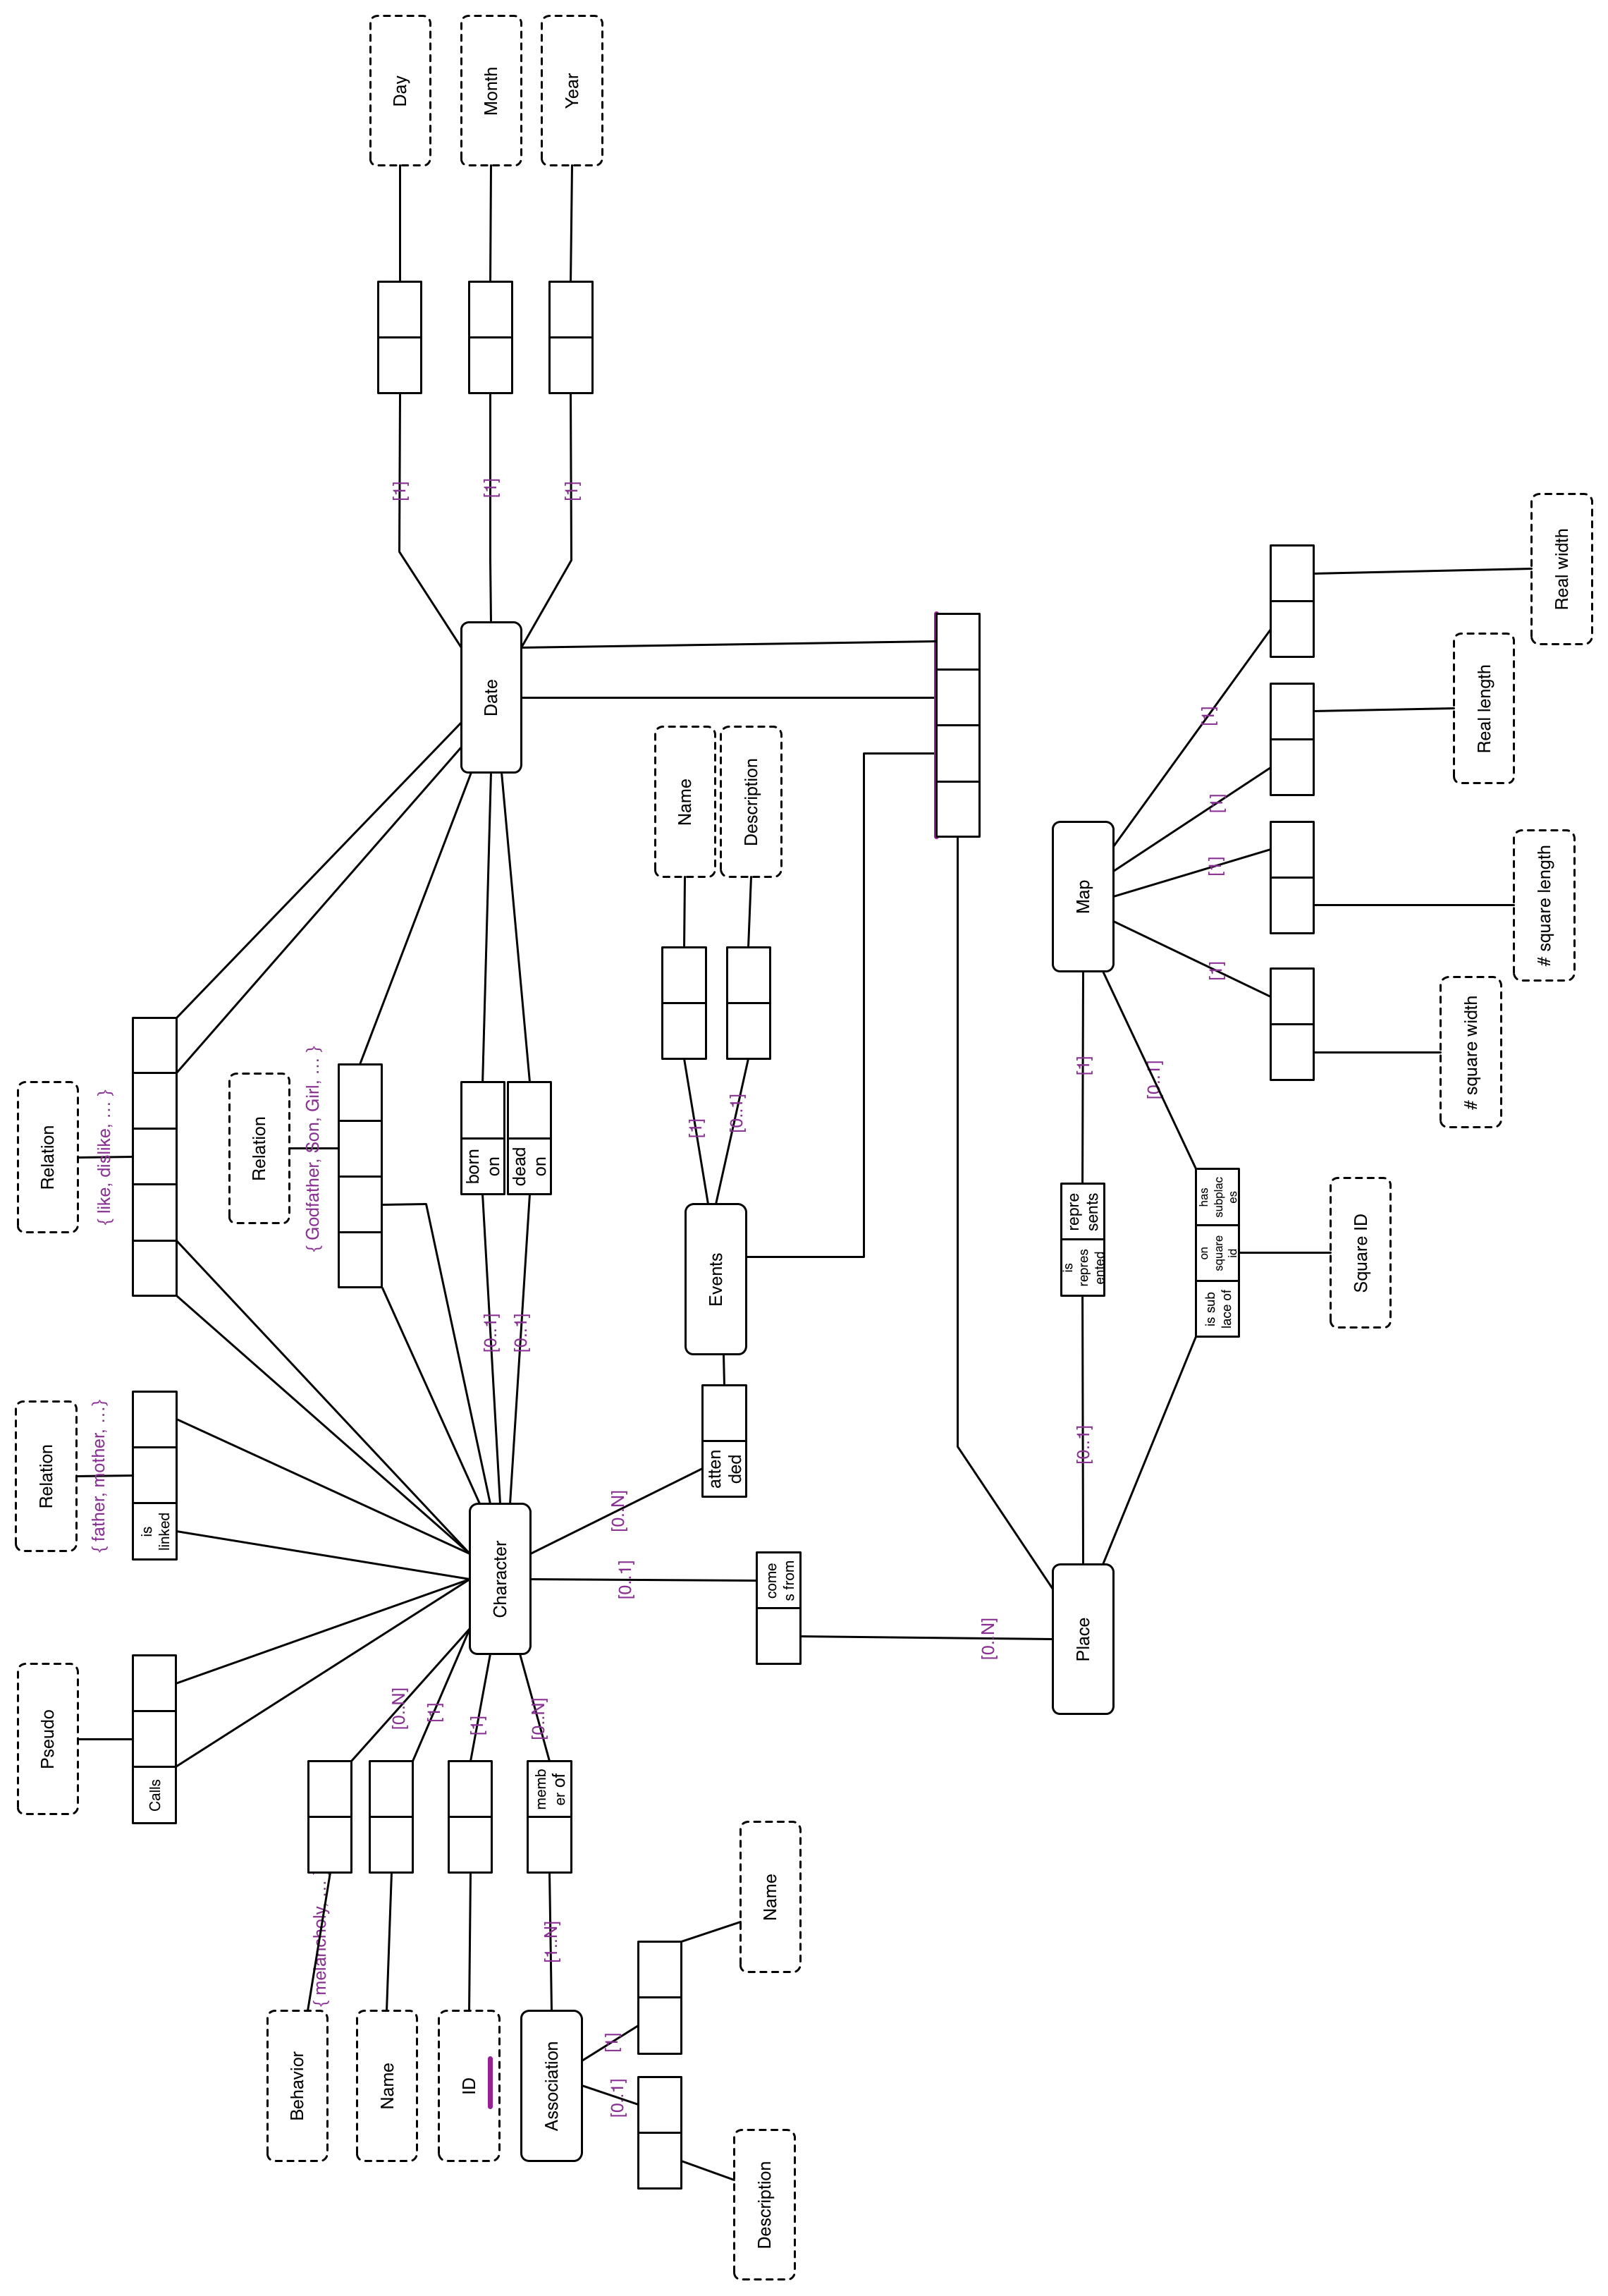
\includegraphics[scale=0.43]{ORM.png}
\caption{ORM Schema}
\label{orm}
\end{figure}

As we can see on the schema, there are 5 main entities which are \texttt{"Characters''}, \texttt{"Date''}, \texttt{"Events''}, \texttt{"Place''}, and \texttt{"Map''}.


We will explain here above three specific case of the diagram :\\

\textbf{Character - Relation relations involving time range, time or timeless notion.} \\
The relations explain the relationships between different characters. They are uni-directional and the different kinds of relations can be defined by the user.
We split these relations into three types to represent the fact that some relations are time-independent (e.g "\dots is my father"), some can start at a given time and be permanent and/or open-ended (e.g "\dots is my godfather since \dots"), and finally some can last for only a while (e.g "\dots was my friend from \dots to \dots").\\

\textbf{Pseudo relation.} \\
This relation involves two characters and a pseudonym. It describes the name used by the first character for the second one. This represents the fact that during the story, a given character might not know another's real name. We added this relation since this can have an impact on the story (he wouldn't realize others were talking about someone he knows for example).
The corresponding table will also allow us the find all the pseudonyms a given person might go by.\\

\textbf{Place - Map relation.} \\
This is a rather complex relation that we introduced to keep track of a story's geography at different levels. The first use is to allow users to situate events or characters. We can also define sub-places to refine locations. 
We can see that a place's map is optional. However, since a place's sub-places are linked to its map, it implicitly  becomes required when we want to add levels. This structure allows us to chain an arbitrary number of levels with a "place - map - place - map - \dots" hierarchy.
This relation has two constraints that are not expressed in the database and will have to be verified in the software implementation. Firstly, the map square on which the sub-place is located must belong to the map's domain of possible squares (between 1 and (\# square width)*(\# square length)). Secondly, it is required that two places of the same level do not overlap.



\end{document}